
%(BEGIN_QUESTION)
% Copyright 2005, Tony R. Kuphaldt, released under the Creative Commons Attribution License (v 1.0)
% This means you may do almost anything with this work of mine, so long as you give me proper credit

The following schematic diagram shows two four-bit universal shift registers used to communicate data serially over a coaxial cable of unspecified length:

$$\includegraphics[width=15.5cm]{i02163x01.eps}$$

Explain how both registers would be used to transmit four bits of parallel data in serial form over the coaxial data cable.

\underbar{file i02163}
%(END_QUESTION)





%(BEGIN_ANSWER)

I won't give you all the details here, but I will get you started with a few steps:

\begin{itemize}
\item{} De-activate the clock enable (CE) inputs of both shift registers.
\item{} Apply the four desired bits (logic levels) to the $D_0$ through $D_3$ inputs of the left-hand shift register.
\item{} Briefly activate the parallel load (PL) input of the left-hand shift register.
\item{} Activate the clock enable (CE) inputs of both shift registers simultaneously for four clock pulses.
\item{} etc.
\item{} etc. . . .
\end{itemize}

%(END_ANSWER)





%(BEGIN_NOTES)

This question asks students to think their way through the operation of two coupled shift registers to accomplish the task of parallel-to-serial-to-parallel data conversion.  Not only is this a good review of shift register operation, but it shows some (not all!) of what happens during the seemingly simple procedure of sending four bits of data in serial form over a cable.

A challenging detail to figure out in this scheme is how to keep both shift registers synchronized so that one receives the serial data bits at the same time the other sends them.  There is more than one way to do this, of course, but the easiest would be to connect the two clock inputs together through another cable conductor.

%INDEX% Electronics review: serial data communication circuit
%INDEX% Electronics review: shift register

%(END_NOTES)


